%%%%%%%%%%%%%%%%%%%%%%%%%%%%%%%%%%%%%%%%%
% Beamer Presentation
% LaTeX Template
% Version 1.0 (10/11/12)
%
% This template has been downloaded from:
% http://www.LaTeXTemplates.com
%
% License:
% CC BY-NC-SA 3.0 (http://creativecommons.org/licenses/by-nc-sa/3.0/)
%
%%%%%%%%%%%%%%%%%%%%%%%%%%%%%%%%%%%%%%%%%

%----------------------------------------------------------------------------------------
%	PACKAGES AND THEMES
%----------------------------------------------------------------------------------------

\documentclass{beamer}

\mode<presentation> {

% The Beamer class comes with a number of default slide themes
% which change the colors and layouts of slides. Below this is a list
% of all the themes, uncomment each in turn to see what they look like.

%\usetheme{default}
%\usetheme{AnnArbor}
%\usetheme{Antibes}
%\usetheme{Bergen}
%\usetheme{Berkeley}
%\usetheme{Berlin}
%\usetheme{Boadilla}
%\usetheme{CambridgeUS}
%\usetheme{Copenhagen}
%\usetheme{Darmstadt}
%\usetheme{Dresden}
%\usetheme{Frankfurt}
%\usetheme{Goettingen}
%\usetheme{Hannover}
%\usetheme{Ilmenau}
%\usetheme{JuanLesPins}
%\usetheme{Luebeck}
%\usetheme{Madrid}
%\usetheme{Malmoe}
%\usetheme{Marburg}
%\usetheme{Montpellier}
%\usetheme{PaloAlto}
%\usetheme{Pittsburgh}
\usetheme{Rochester}
%\usetheme{Singapore}
%\usetheme{Szeged}
%\usetheme{Warsaw}

% As well as themes, the Beamer class has a number of color themes
% for any slide theme. Uncomment each of these in turn to see how it
% changes the colors of your current slide theme.

%\usecolortheme{albatross}
%\usecolortheme{beaver}
%\usecolortheme{beetle}
%\usecolortheme{crane}
%\usecolortheme{dolphin}
%\usecolortheme{dove}
%\usecolortheme{fly}
%\usecolortheme{lily}
%\usecolortheme{orchid}
%\usecolortheme{rose}
%\usecolortheme{seagull}
%\usecolortheme{seahorse}
%\usecolortheme{whale}
%\usecolortheme{wolverine}

%\setbeamertemplate{footline} % To remove the footer line in all slides uncomment this line
%\setbeamertemplate{footline}[page number] % To replace the footer line in all slides with a simple slide count uncomment this line

\setbeamertemplate{navigation symbols}{} % To remove the navigation symbols from the bottom of all slides uncomment this line

\definecolor{OUGold}{RGB}{181,154,57}
\setbeamercolor{structure}{fg=OUGold}
\setbeamercolor{block title example}{bg=OUGold}
\setbeamercolor{section in toc}{fg=black}

% position the logo
\addtobeamertemplate{frametitle}{}{%
	\begin{textblock*}{\paperwidth}(290pt,-38pt)
		
\includegraphics[height=1cm,keepaspectratio]{sail}
	\end{textblock*}}
}

\usepackage{textpos} % package for the positioning
\usepackage{graphicx} % Allows including images
\usepackage{booktabs} % Allows the use of \toprule, \midrule and \bottomrule in tables
\usepackage{pdfpages} % Allows including PDFs (in separate frame)

%----------------------------------------------------------------------------------------
%	TITLE PAGE
%----------------------------------------------------------------------------------------

\title[Bank Marketing Project]{Bank Marketing Project: Presentation 1} % The short title appears at the bottom of every slide, the full title is only on the title page

\author{Evan Bradley} % Your name
\institute[OU] % Your institution as it will appear on the bottom of every slide, may be shorthand to save space
{
Oakland University \\ % Your institution for the title page
\medskip
\textit{edbradley@oakland.edu} % Your email address
}
\date{October 2016} % Date, can be changed to a custom date

\begin{document}

\begin{frame}
	\frametitle{\space}
	\titlepage % Print the title page as the first slide
\end{frame}

\begin{frame}
\frametitle{Overview} % Table of contents slide, comment this block out to remove it
\tableofcontents % Throughout your presentation, if you choose to use \section{} and \subsection{} commands, these will automatically be printed on this slide as an overview of your presentation
\end{frame}

%----------------------------------------------------------------------------------------
%	PRESENTATION SLIDES
%----------------------------------------------------------------------------------------

%------------------------------------------------
\section{Overview of Variables} % Sections can be created in order to organize your presentation into discrete blocks, all sections and subsections are automatically printed in the table of contents as an overview of the talk
%------------------------------------------------

%\subsection{Test} % A subsection can be created just before a set of slides with a common theme to further break down your presentation into chunks

%------------------------------------------------

\begin{frame}
	\frametitle{Overview of Numeric Variables}
  \begin{columns}[c]
	\column{.45\textwidth} % Left column and width
	\begin{itemize}
		\item Age
		\newline
		\item Duration of phone call
		\newline
		\item Number of previous contacts
		\newline
		\item Days since previously contacted
		\newline
		\item Number of contacts
		\newline
	\end{itemize}

	\column{.45\textwidth} % Left column and width
	\begin{itemize}
		\item Employment Variation Rate
		\newline
		\item Consumer Price Index
		\newline
		\item Consumer Confidence Index
		\newline
		\item Euribor 3-month Rate
		\newline
		\item Number of employees
		\newline
	\end{itemize}
  \end{columns}
\end{frame}

% ------------------------------------------------
\section{Basic Analysis of Numeric Data} % Sections can be created in order to organize your presentation into discrete blocks, all sections and subsections are automatically printed in the table of contents as an overview of the talk
%------------------------------------------------

\begin{frame}
	\frametitle{Age}
	\begin{columns}[c] % The "c" option specifies centered vertical alignment while the "t" option is used for top vertical alignment
		
		\column{.35\textwidth} % Left column and width
    Yes:
		\begin{itemize}
			\item Median: 37
			\item Mean: 40.91
      \item SD: 13.83748
		\end{itemize}
		
		\column{.40\textwidth} % Right column and width
    No:
		\begin{itemize}
			\item Median: 38
			\item Mean: 39.91
      \item SD: 9.898132
		\end{itemize}
		
	\end{columns}
\end{frame}

\begin{frame}
	\frametitle{Number of Contacts}
	\begin{columns}[c] % The "c" option specifies centered vertical alignment while the "t" option is used for top vertical alignment
		
		\column{.35\textwidth} % Left column and width
    Yes:
		\begin{itemize}
			\item Median: 2.0
			\item Mean: 2.052
      \item SD: 1.666245
		\end{itemize}
		
		\column{.40\textwidth} % Right column and width
    No:
		\begin{itemize}
			\item Median: 2.0
			\item Mean: 2.633 
      \item SD: 2.873438
		\end{itemize}
		
	\end{columns}
\end{frame}

\begin{frame}
	\frametitle{Days Since Previously Contacted}
	\begin{columns}[c] % The "c" option specifies centered vertical alignment while the "t" option is used for top vertical alignment
		
		\column{.35\textwidth} % Left column and width
    Yes:
		\begin{itemize}
			\item Median: 999
			\item Mean: 792
      \item SD: 403.4072
		\end{itemize}
		
		\column{.40\textwidth} % Right column and width
    No:
		\begin{itemize}
			\item Median: 999
			\item Mean: 984.1
      \item SD: 120.6569
		\end{itemize}
		
	\end{columns}
\end{frame}

\begin{frame}
	\frametitle{Number of Previous Contacts}
	\begin{columns}[c] % The "c" option specifies centered vertical alignment while the "t" option is used for top vertical alignment
		
		\column{.35\textwidth} % Left column and width
    Yes:
		\begin{itemize}
			\item Median: 0
			\item Mean: 0.4927
      \item SD: 0.8603441
		\end{itemize}
		
		\column{.40\textwidth} % Right column and width
    No:
		\begin{itemize}
			\item Median: 0
			\item Mean: 0.1324
      \item SD: 0.4091992
		\end{itemize}
		
	\end{columns}
\end{frame}

\begin{frame}
	\frametitle{Employment Variation Rate}
	\begin{columns}[c] % The "c" option specifies centered vertical alignment while the "t" option is used for top vertical alignment
		
		\column{.35\textwidth} % Left column and width
    Yes:
		\begin{itemize}
			\item Median: -1.800
			\item Mean: -1.233
      \item SD: 1.623626
		\end{itemize}
		
		\column{.40\textwidth} % Right column and width
    No:
		\begin{itemize}
			\item Median: 1.1000
			\item Mean: 0.2489
      \item SD: 1.482932
		\end{itemize}
		
	\end{columns}
\end{frame}

\begin{frame}
	\frametitle{Consumer Price Index}
	\begin{columns}[c] % The "c" option specifies centered vertical alignment while the "t" option is used for top vertical alignment
		
		\column{.35\textwidth} % Left column and width
    Yes:
		\begin{itemize}
			\item Median: 93.20
			\item Mean: 93.35 
      \item SD: 1.482932
		\end{itemize}
		
		\column{.40\textwidth} % Right column and width
    No:
		\begin{itemize}
			\item Median: 93.92
			\item Mean: 93.60
      \item SD: 0.5589929
		\end{itemize}
		
	\end{columns}
\end{frame}

\begin{frame}
	\frametitle{Consumer Confidence Index}
	\begin{columns}[c] % The "c" option specifies centered vertical alignment while the "t" option is used for top vertical alignment
		
		\column{.35\textwidth} % Left column and width
    Yes:
		\begin{itemize}
			\item Median: -40.40
			\item Mean: -39.79
      \item SD: 6.139668
		\end{itemize}
		
		\column{.40\textwidth} % Right column and width
    No:
		\begin{itemize}
			\item Median: -41.80
			\item Mean: -40.59
      \item SD: 4.391155
		\end{itemize}
		
	\end{columns}
\end{frame}

\begin{frame}
	\frametitle{Euro Interbank Offer Rate for 3 Months}
	\begin{columns}[c] % The "c" option specifies centered vertical alignment while the "t" option is used for top vertical alignment
		
		\column{.35\textwidth} % Left column and width
    Yes:
		\begin{itemize}
			\item Median: 1.266
			\item Mean: 2.123
      \item SD: 1.742598
		\end{itemize}
		
		\column{.40\textwidth} % Right column and width
    No:
		\begin{itemize}
			\item Median: 4.857
			\item Mean: 3.811
      \item SD: 1.638187
		\end{itemize}
		
	\end{columns}
\end{frame}

\begin{frame}
	\frametitle{Number of Employees}
	\begin{columns}[c] % The "c" option specifies centered vertical alignment while the "t" option is used for top vertical alignment
		
		\column{.35\textwidth} % Left column and width
    Yes:
		\begin{itemize}
			\item Median: 5099
			\item Mean: 5095
      \item SD: 87.57264
		\end{itemize}
		
		\column{.40\textwidth} % Right column and width
    No:
		\begin{itemize}
			\item Median: 5196
			\item Mean: 5176
      \item SD: 64.57198
		\end{itemize}
		
	\end{columns}
\end{frame}

\begin{frame}
  \frametitle{Graph of Numeric Variables}
	\begin{columns}[c] % The "c" option specifies centered vertical alignment while the "t" option is used for top vertical alignment
		\column{.65\textwidth}
    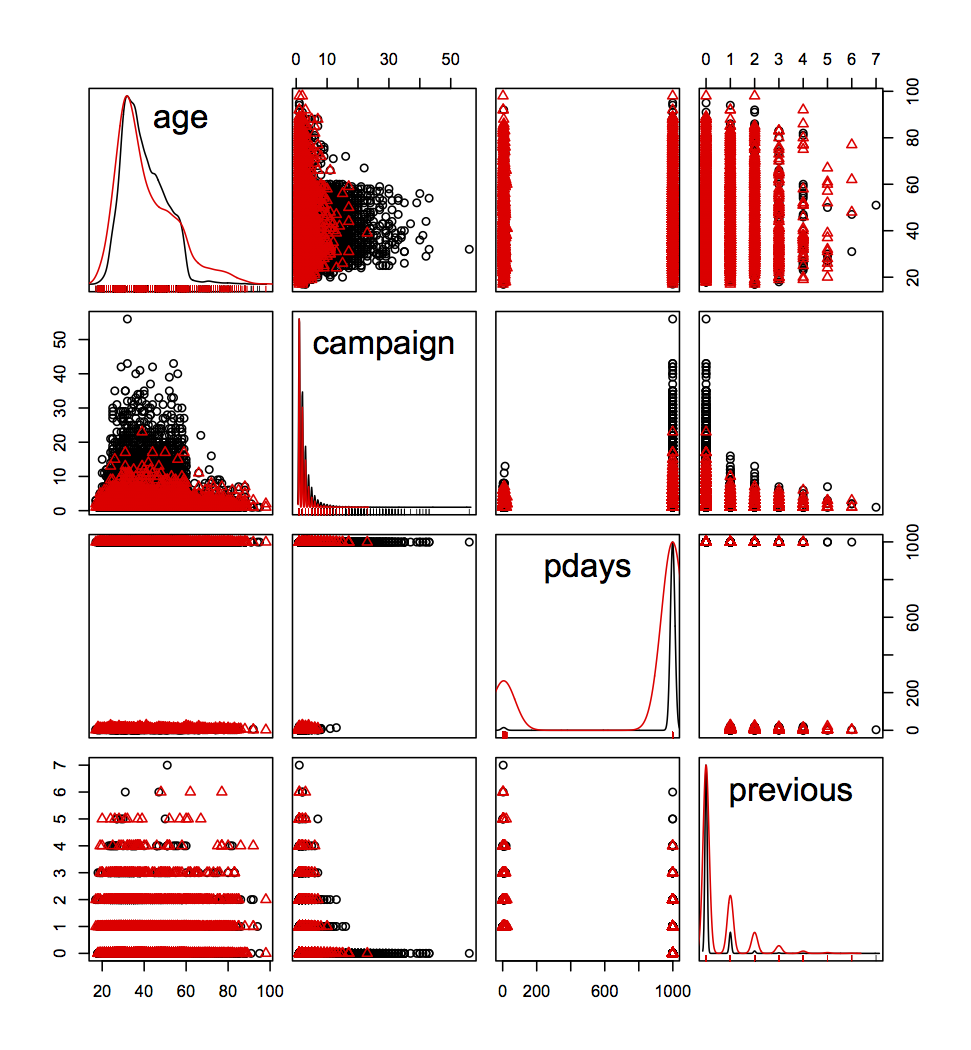
\includegraphics[height=\textheight]{matrix1}
  \end{columns}
\end{frame}


\begin{frame}
  \frametitle{Graph of Numeric Variables}
	\begin{columns}[c] % The "c" option specifies centered vertical alignment while the "t" option is used for top vertical alignment
		\column{.65\textwidth}
    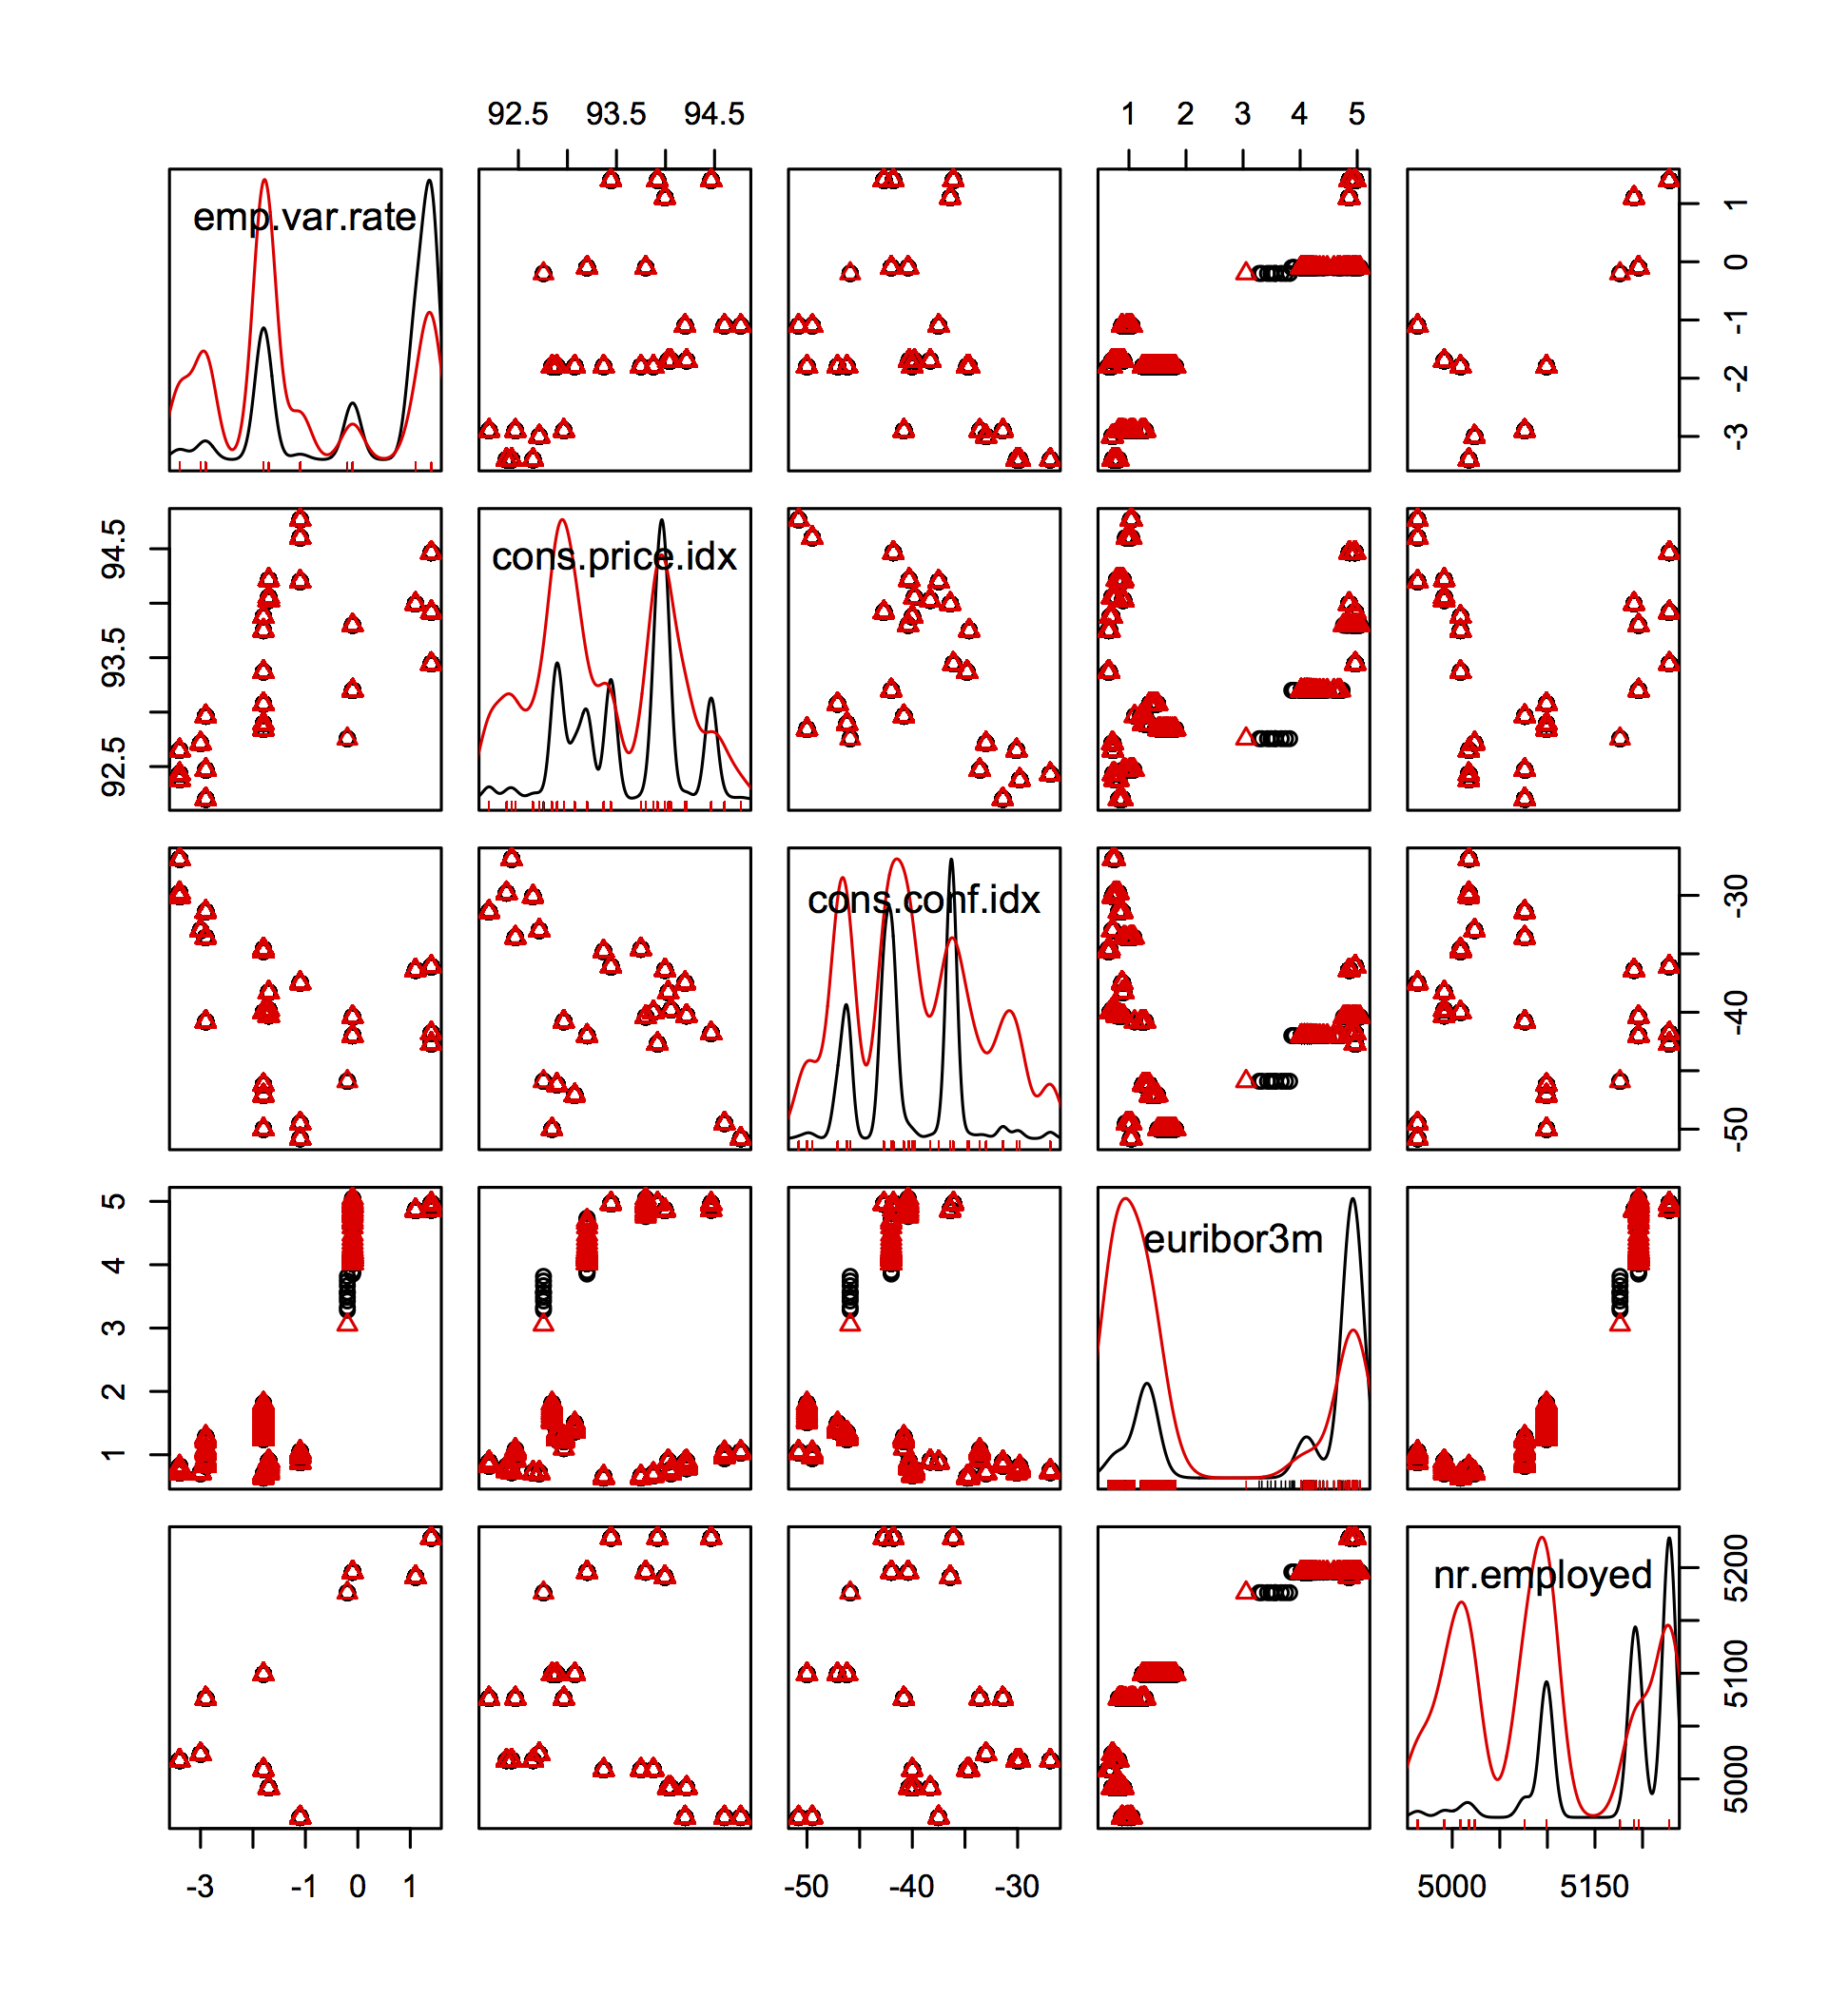
\includegraphics[height=\textheight]{matrix2}
  \end{columns}
\end{frame}

%------------------------------------------------
\section{Overview of Categorical Variables}
%------------------------------------------------

\begingroup
\small
\begin{frame}[fragile]
  \frametitle{Job Type}
  \begin{verbatim}
              y
job               no  yes
  admin.        9070 1352
  blue-collar   8616  638
  entrepreneur  1332  124
  housemaid      954  106
  management    2596  328
  retired       1286  434
  self-employed 1272  149
  services      3646  323
  student        600  275
  technician    6013  730
  unemployed     870  144
  unknown        293   37

X-squared = 961.24, df = 11, p-value < 2.2e-16
  \end{verbatim}
\end{frame}
\endgroup

\begin{frame}[fragile]
  \frametitle{Marital Status}
  \begin{verbatim}
marital       no   yes
  divorced  4136   476
  married  22396  2532
  single    9948  1620
  unknown     68    12

X-squared = 122.66, df = 3, p-value < 2.2e-16
  \end{verbatim}
\end{frame}

\begin{frame}[fragile]
  \frametitle{Level of Education}
  \begin{verbatim}
                     y
education                no   yes
  basic.4y             3748   428
  basic.6y             2104   188
  basic.9y             5572   473
  high.school          8484  1031
  illiterate             14     4
  professional.course  4648   595
  university.degree   10498  1670
  unknown              1480   251

X-squared = 193.11, df = 7, p-value < 2.2e-16
  \end{verbatim}
\end{frame}

\begin{frame}[fragile]
  \frametitle{Default on Credit}
  \begin{verbatim}
         y
default      no   yes
  no      28391  4197
  unknown  8154   443
  yes         3     0

X-squared = 406.58, df = 2, p-value < 2.2e-16
  \end{verbatim}
\end{frame}

\begin{frame}[fragile]
  \frametitle{Housing Loan}
  \begin{verbatim}
        y
housing      no   yes
  no      16596  2026
  unknown   883   107
  yes     19069  2507

X-squared = 5.6845, df = 2, p-value = 0.05829
  \end{verbatim}
\end{frame}

\begin{frame}[fragile]
  \frametitle{Personal Loan}
  \begin{verbatim}
         y
loan         no   yes
  no      30100  3850
  unknown   883   107
  yes      5565   683

X-squared = 1.094, df = 2, p-value = 0.5787
  \end{verbatim}
\end{frame}

\begin{frame}[fragile]
  \frametitle{Contact Type}
  \begin{verbatim}
           y
contact        no   yes
  cellular  22291  3853
  telephone 14257   787

X-squared = 862.32, df = 1, p-value < 2.2e-16
  \end{verbatim}
\end{frame}

\begin{frame}[fragile]
  \frametitle{Month of Call}
  \begin{verbatim}
     y
month    no   yes
  apr  2093   539
  aug  5523   655
  dec    93    89
  jul  6525   649
  jun  4759   559
  mar   270   276
  may 12883   886
  nov  3685   416
  oct   403   315
  sep   314   256

X-squared = 3101.1, df = 9, p-value < 2.2e-16
  \end{verbatim}
\end{frame}

\begin{frame}[fragile]
  \frametitle{Day of Week}
  \begin{verbatim}
           y
day_of_week   no  yes
        fri 6981  846
        mon 7667  847
        thu 7578 1045
        tue 7137  953
        wed 7185  949

X-squared = 26.145, df = 4, p-value = 2.958e-05
  \end{verbatim}
\end{frame}

\begin{frame}[fragile]
  \frametitle{Previous Campaign Outcome}
  \begin{verbatim}
             y
poutcome         no   yes
  failure      3647   605
  nonexistent 32422  3141
  success       479   894

X-squared = 4230.5, df = 2, p-value < 2.2e-16
  \end{verbatim}
\end{frame}

%------------------------------------------------
\section{Classification Models}
%------------------------------------------------

\begin{frame}
  \frametitle{Classification Model Ideas}
  \begin{itemize}
    \item Decision Tree
      \newline
    \item Neural Net
      \newline
    \item Support Vector Machine
      \newline
  \end{itemize}
\end{frame}

\begin{frame}
  \frametitle{Decision Tree}
	\begin{columns}[c] % The "c" option specifies centered vertical alignment while the "t" option is used for top vertical alignment
		\column{.75\textwidth}
    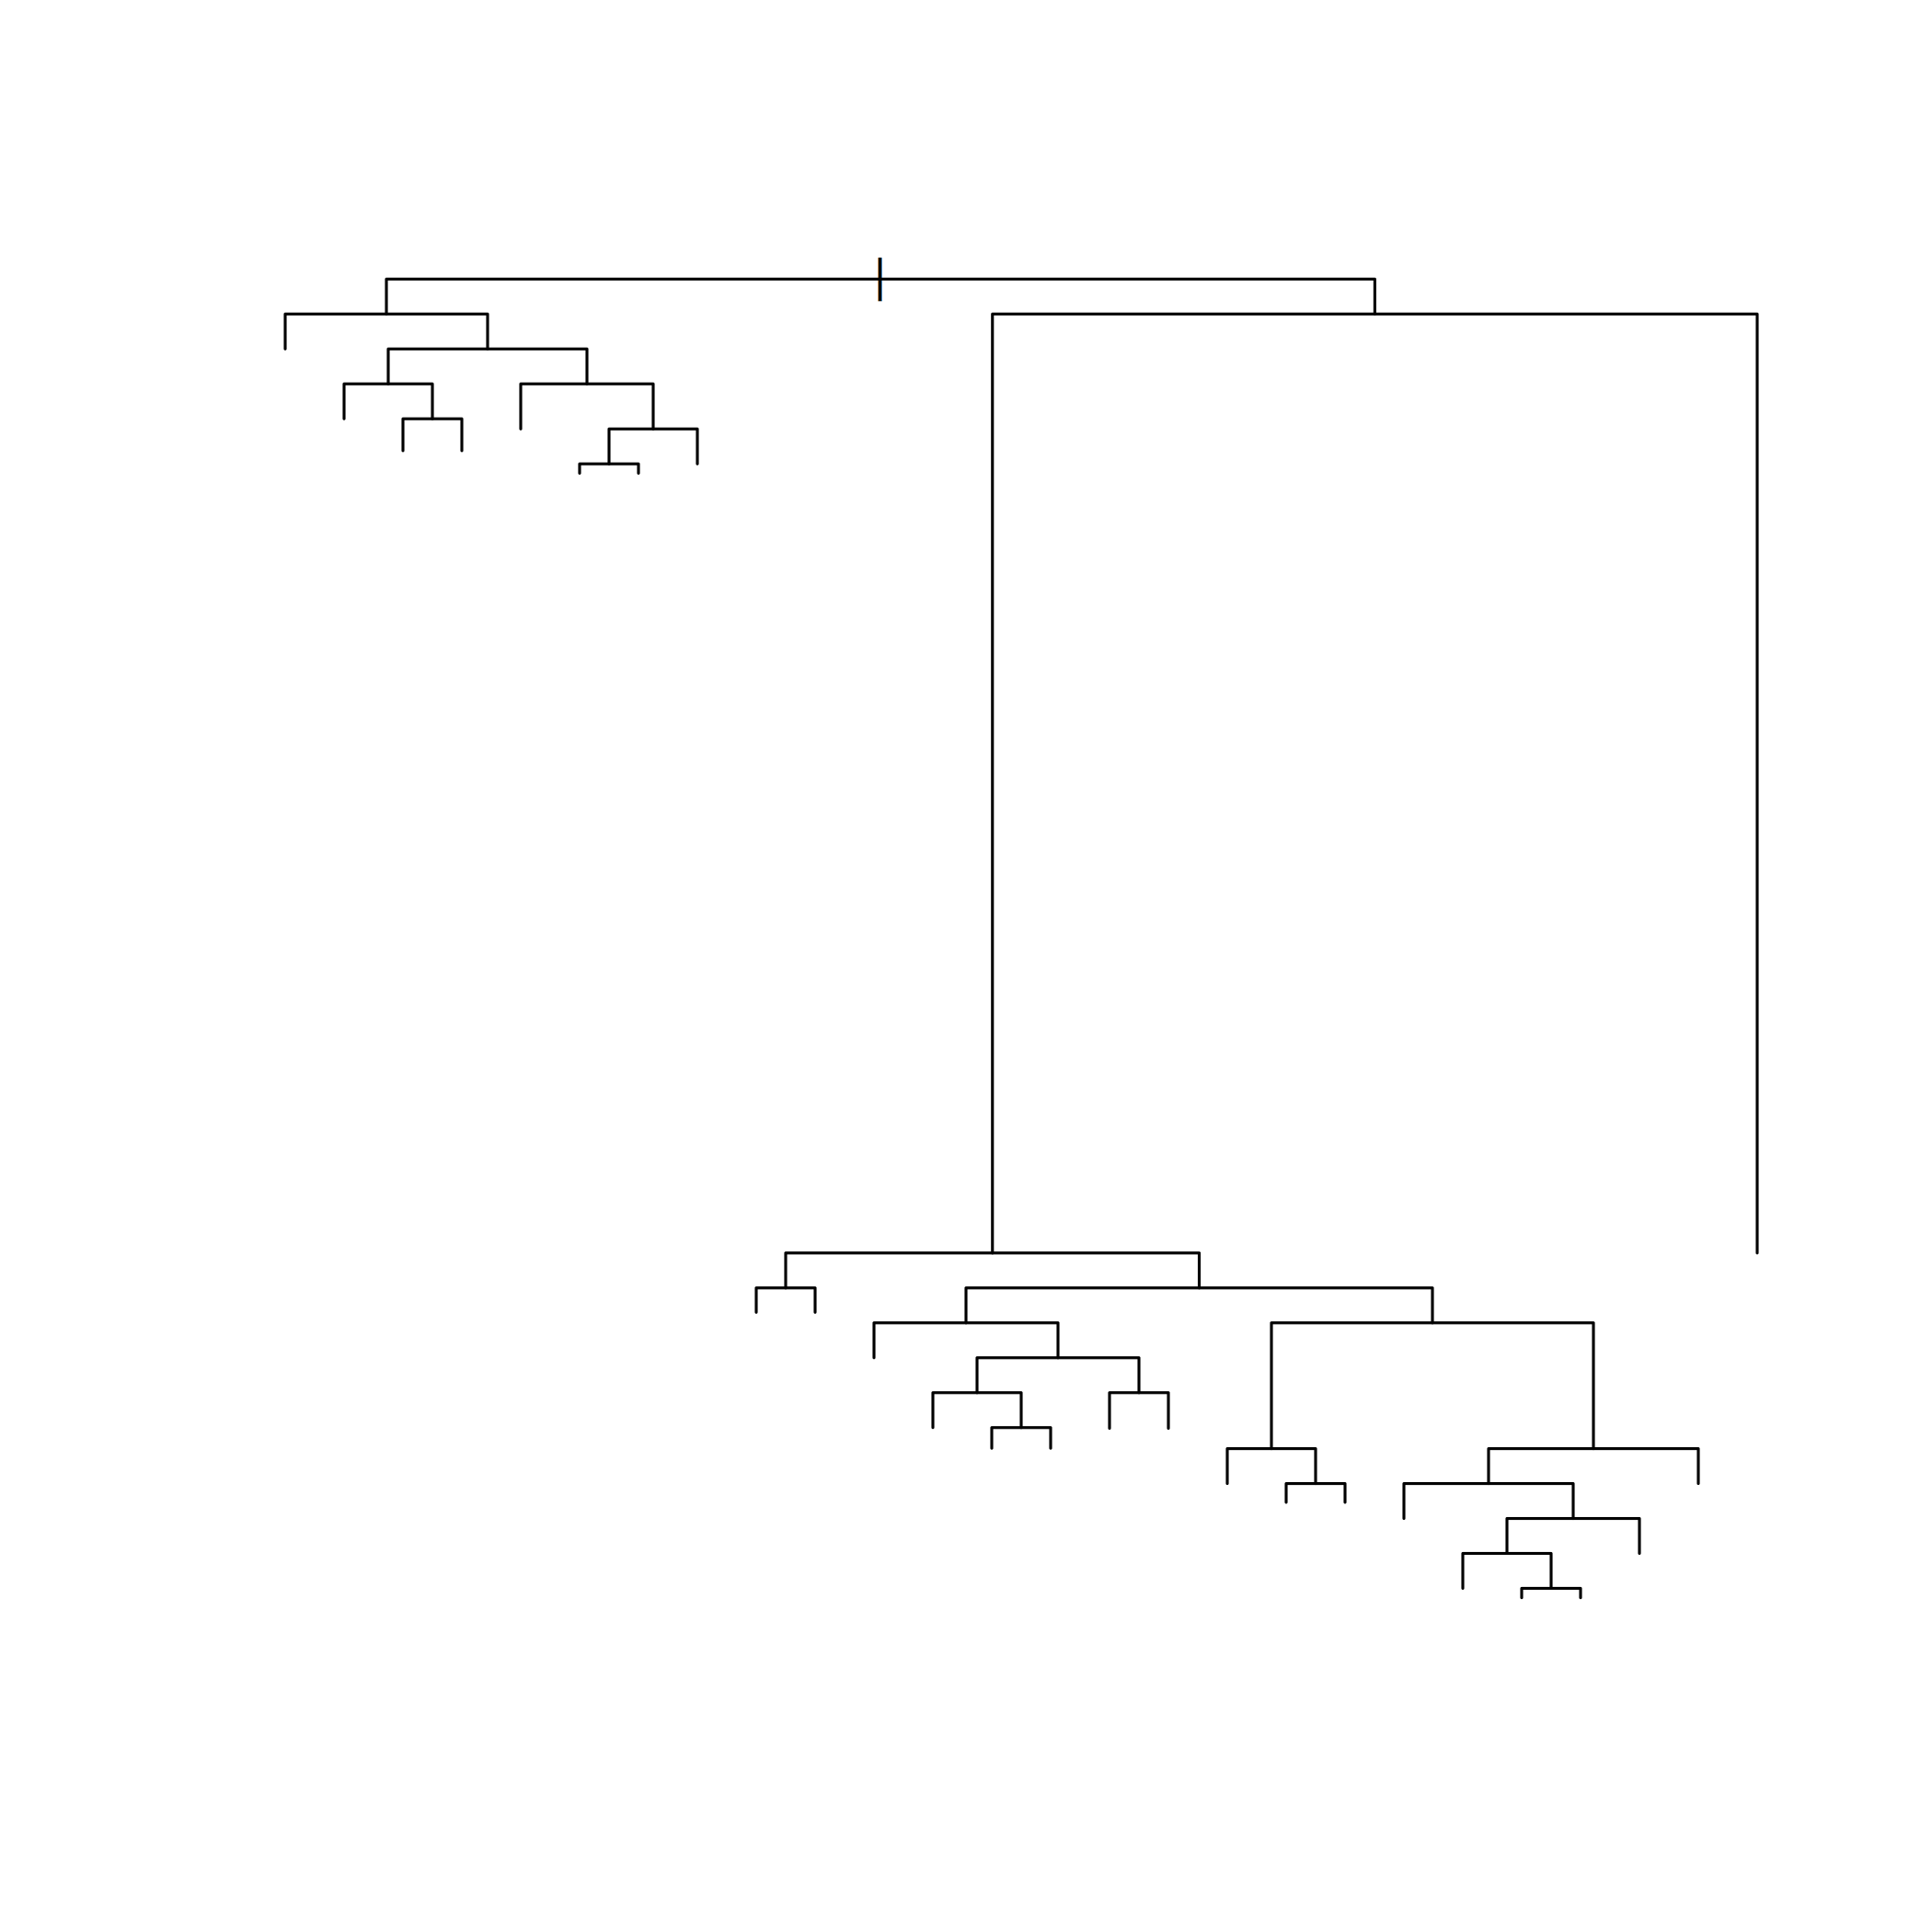
\includegraphics[height=\textheight]{tree}
  \end{columns}
\end{frame}


\begin{frame}
  \frametitle{Labeled Decision Tree}
	\begin{columns}[c] % The "c" option specifies centered vertical alignment while the "t" option is used for top vertical alignment
		\column{.75\textwidth}
    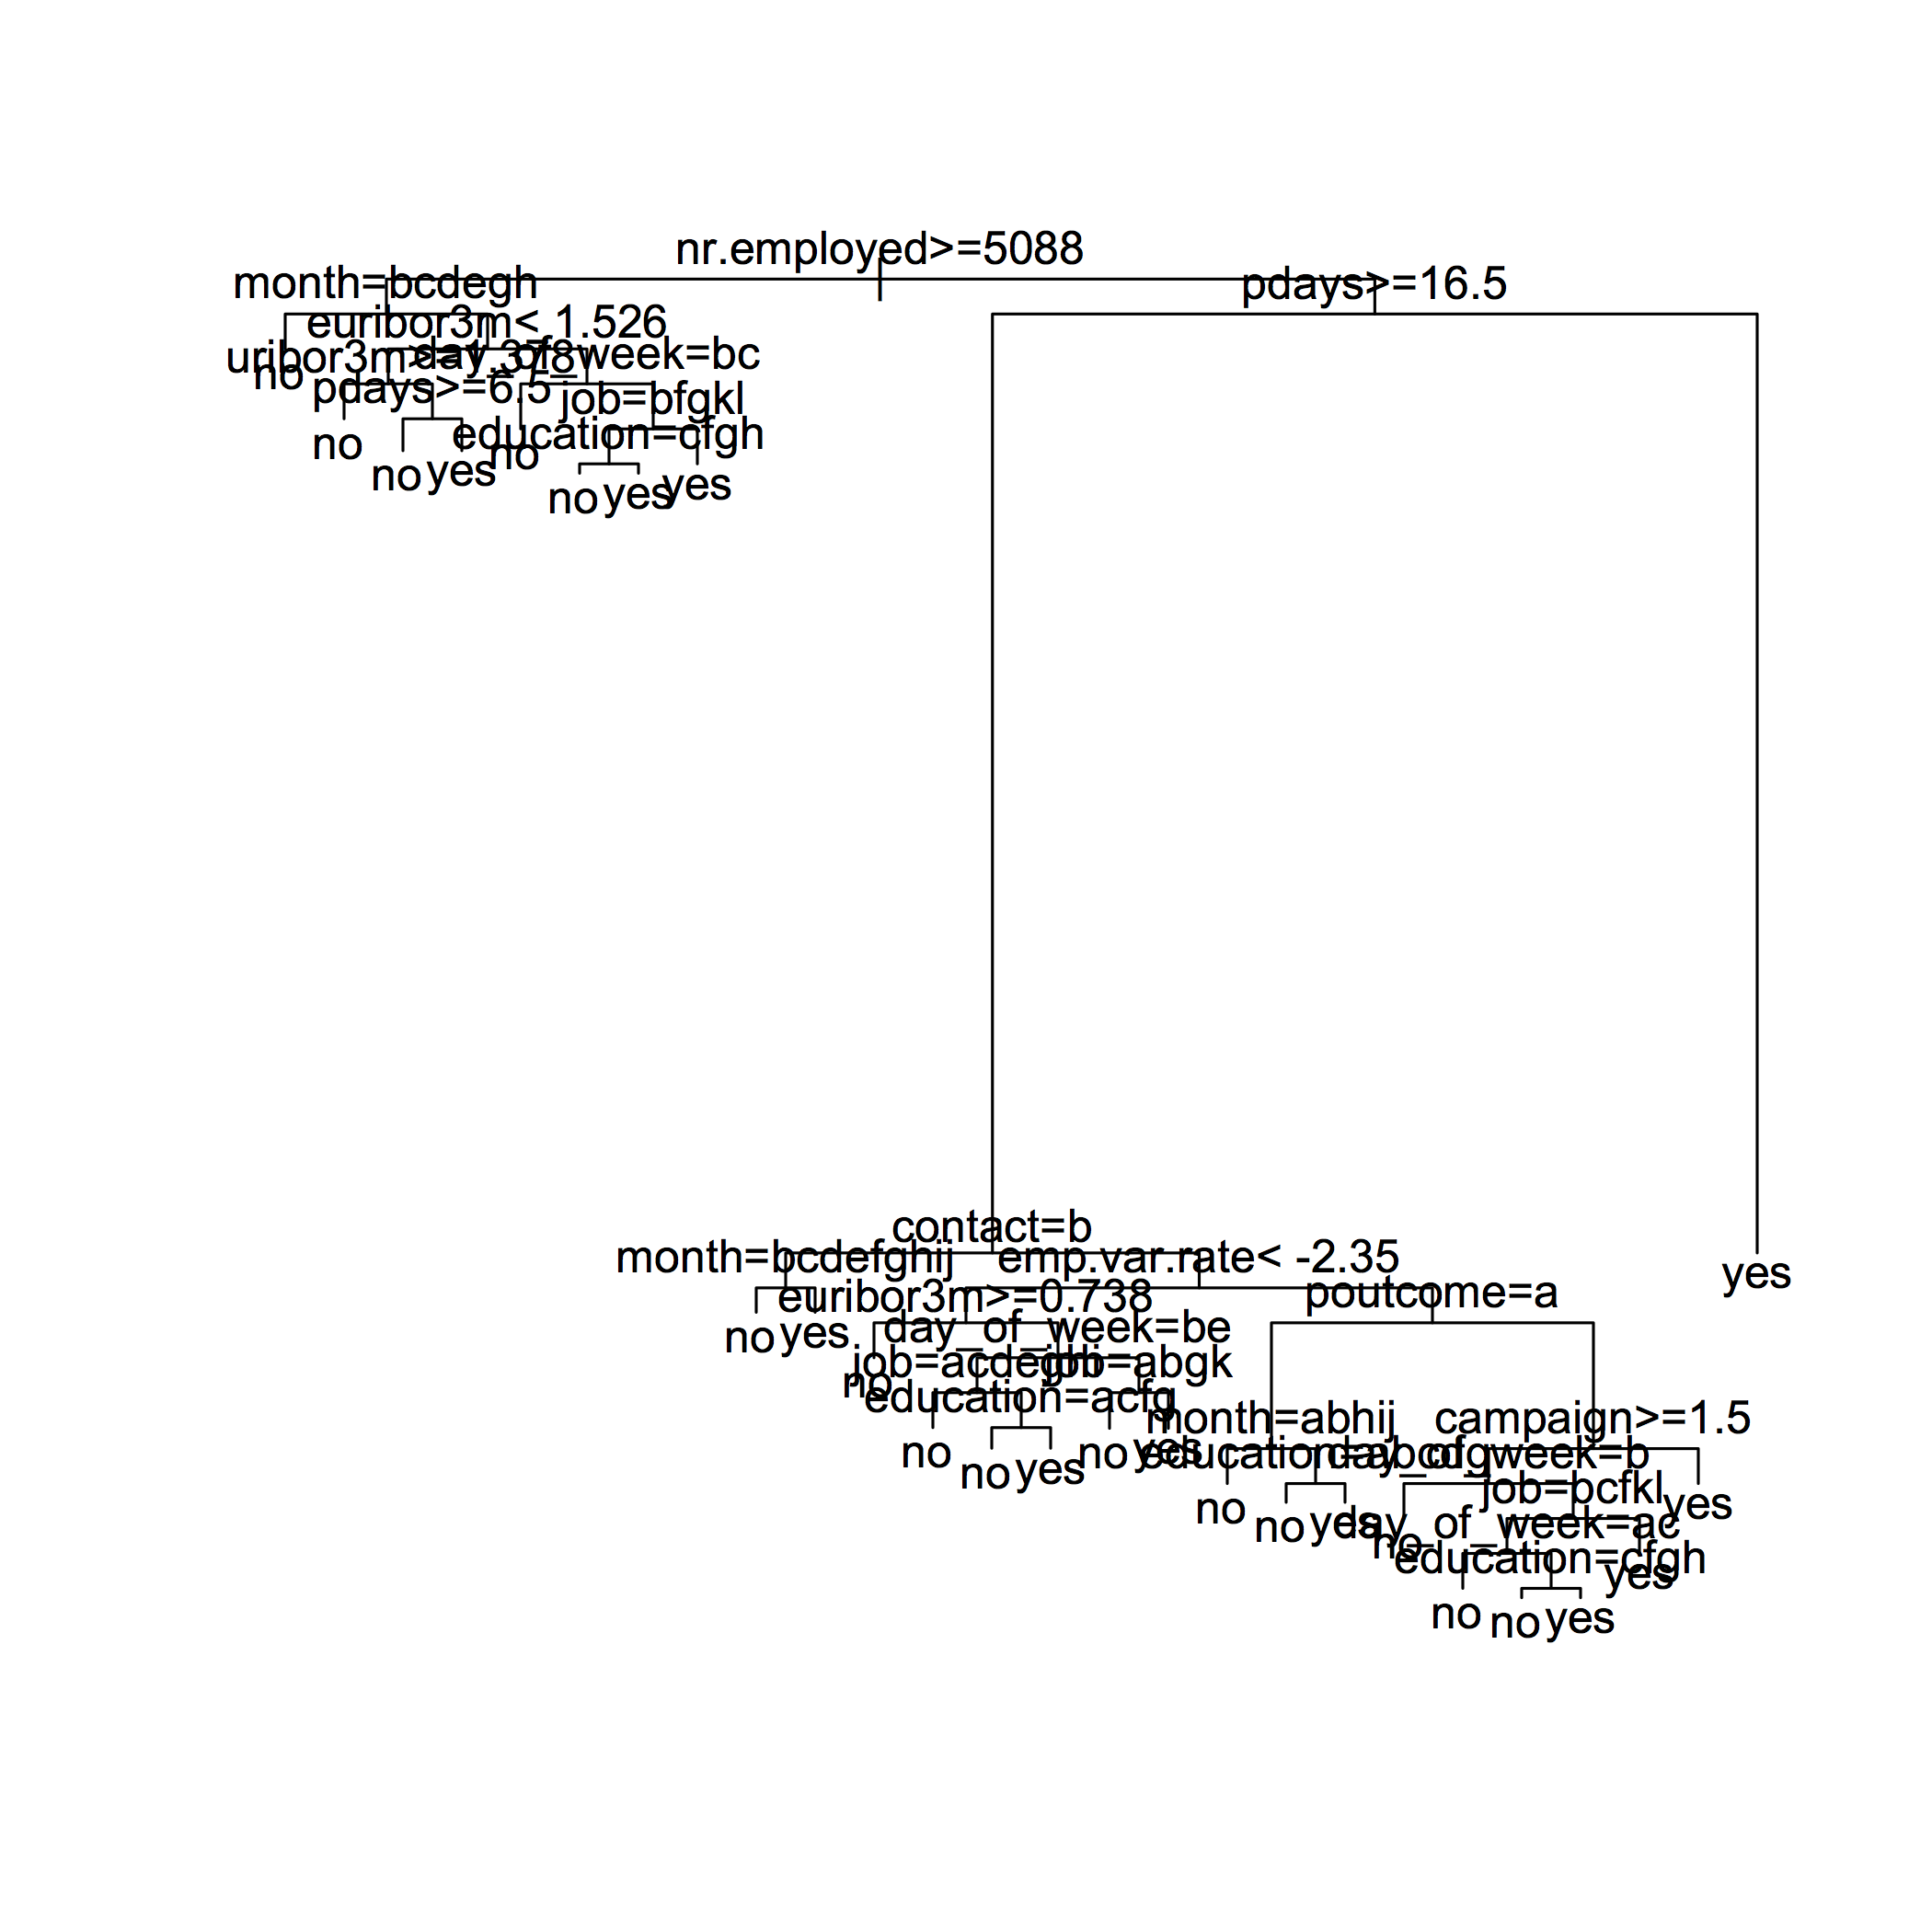
\includegraphics[height=\textheight]{labeled_tree}
  \end{columns}
\end{frame}

\begin{frame}
  \frametitle{Cross Validation of Decision Tree}
	\begin{columns}[c] % The "c" option specifies centered vertical alignment while the "t" option is used for top vertical alignment
		\column{.75\textwidth}
    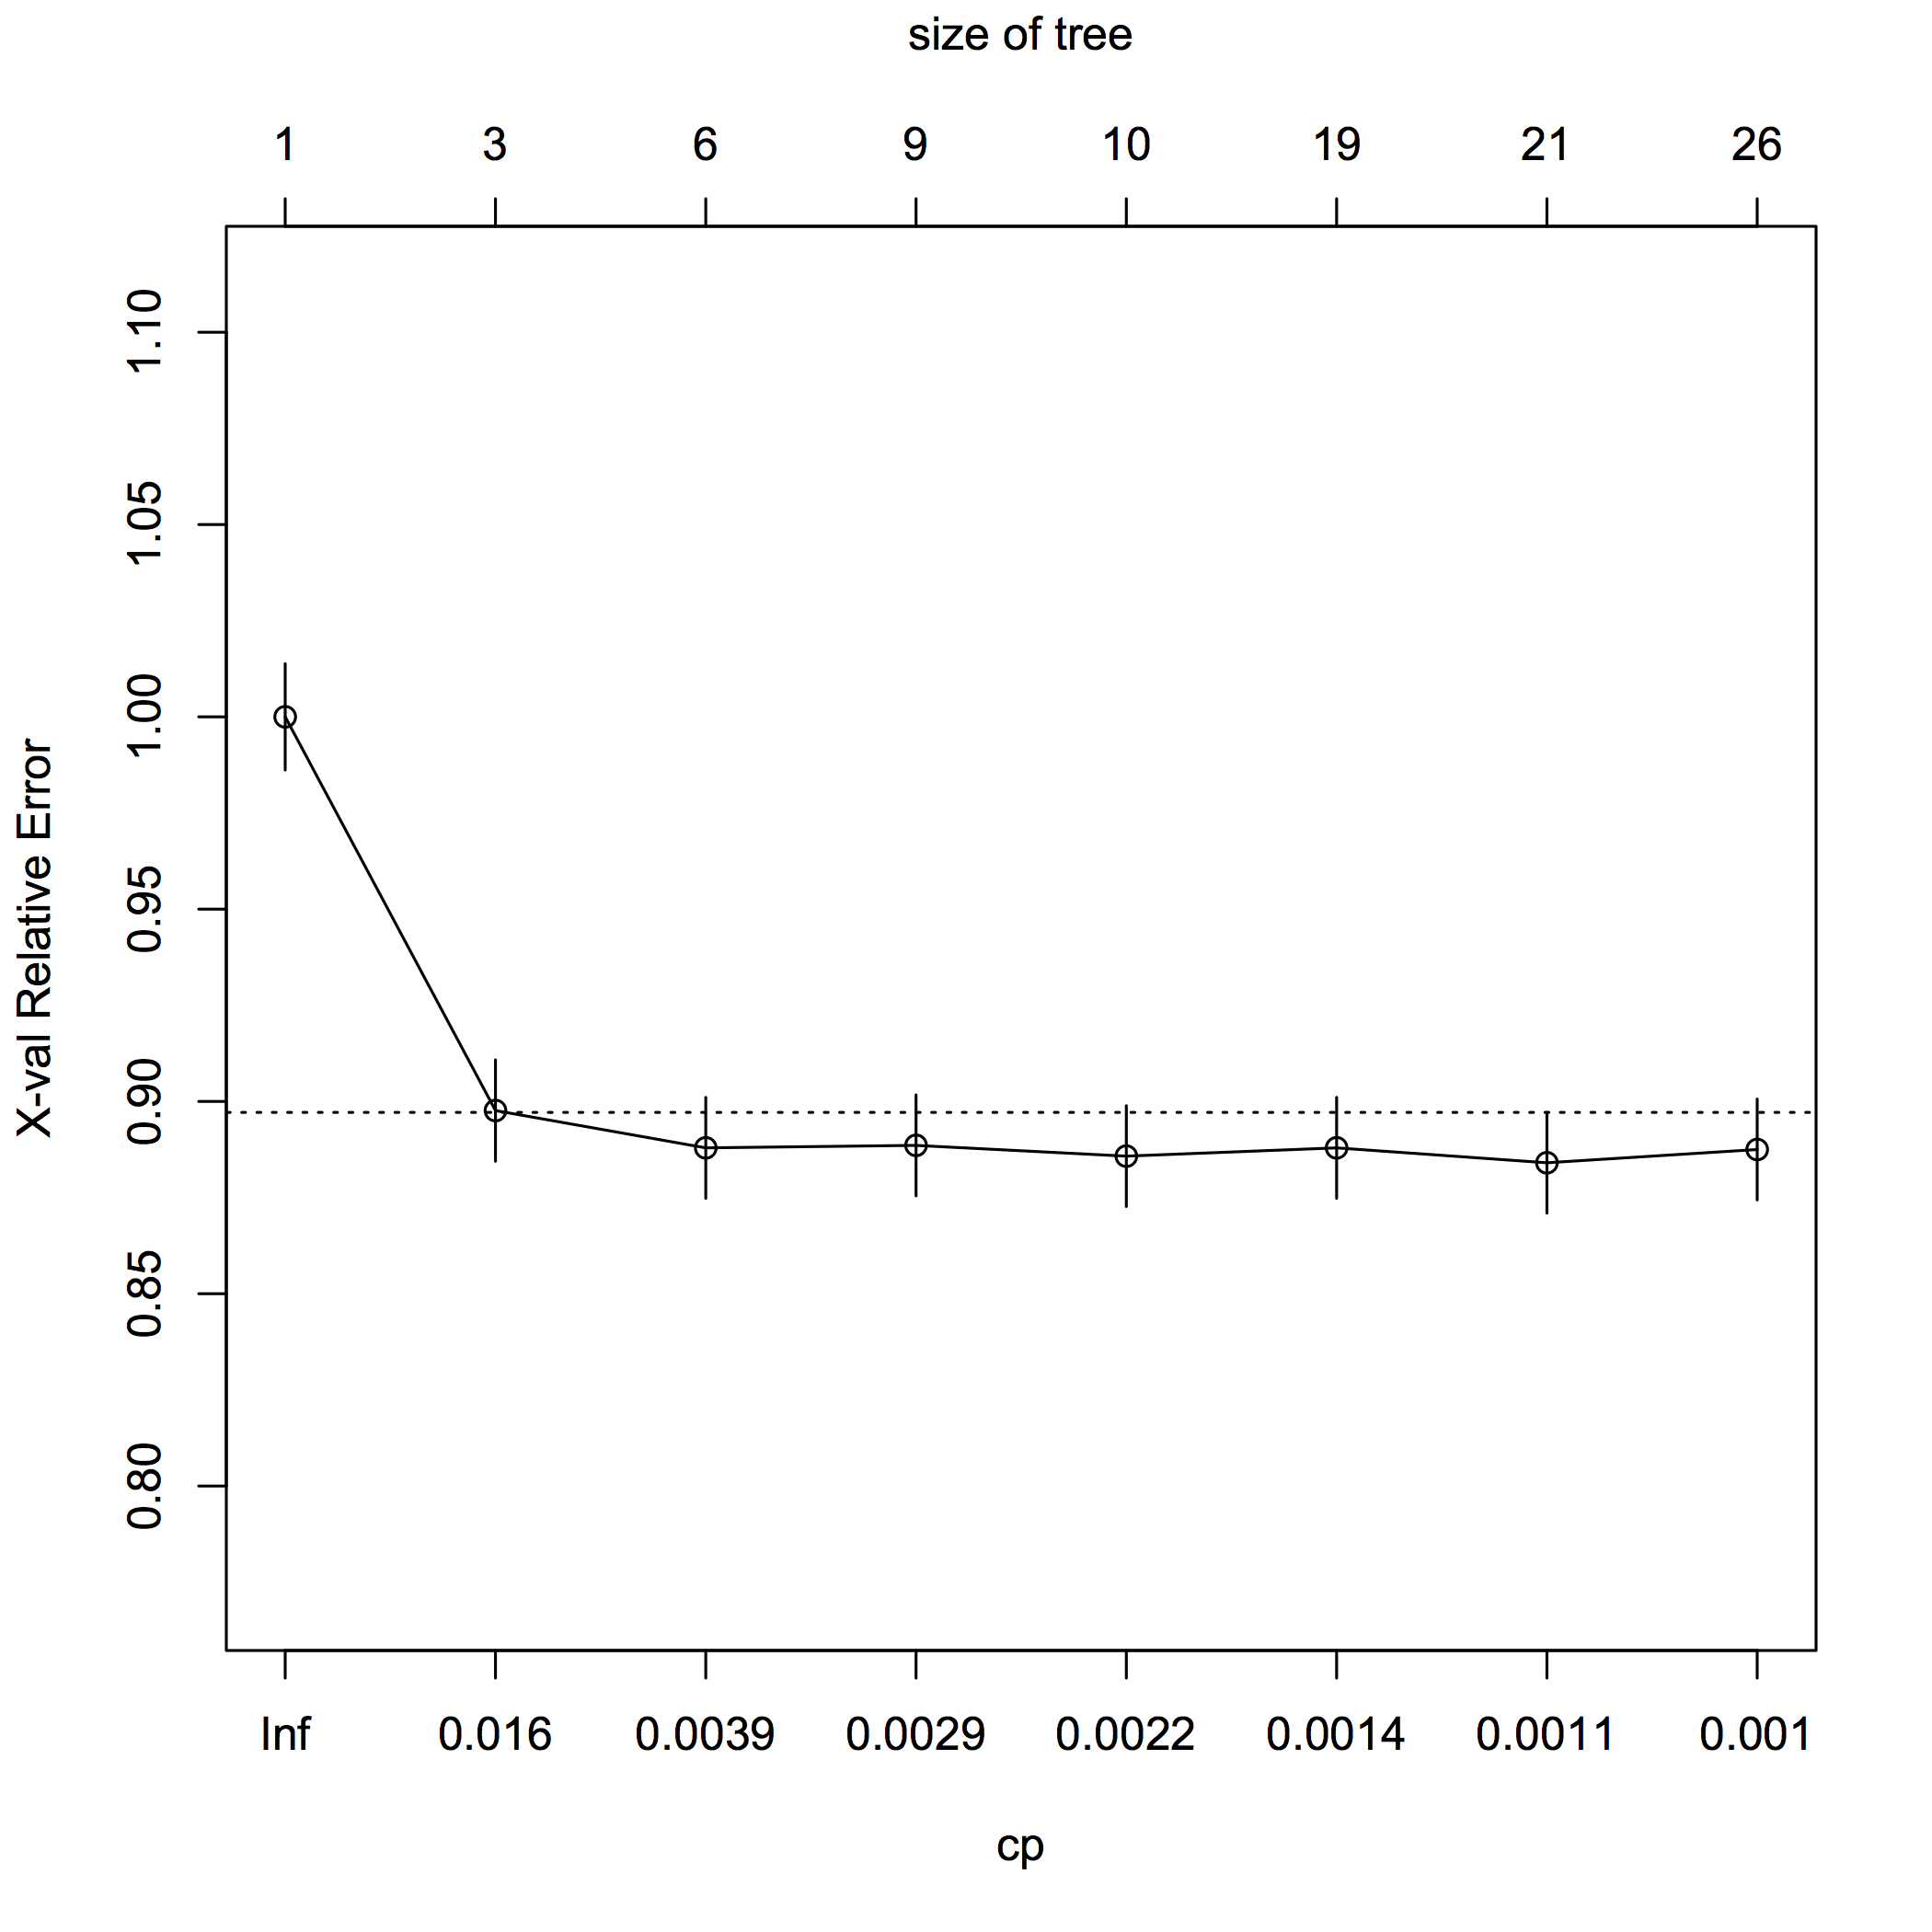
\includegraphics[height=\textheight]{accuracy}
  \end{columns}
\end{frame}

%----------------------------------------------------------------------------------------

\end{document} 